\documentclass[10pt,a4paper,sans]{moderncv}
    \moderncvstyle{banking}
    \moderncvcolor{black}
    \nopagenumbers{}

    \usepackage[utf8]{inputenc}
    \usepackage[top=0.15cm, bottom=0.15cm, left=0.25cm, right=0.25cm]{geometry}
    \usepackage{ragged2e}
    \usepackage{multicol}
    \usepackage{enumitem}
    \usepackage{amssymb}
    \usepackage{fontawesome5}
    \usepackage{xcolor}
    \usepackage{hyperref}
    \hypersetup{colorlinks=true, urlcolor=blue}

    % Custom cventry
    \newcommand*{\customcventry}[7][.10em]{%
    \begin{tabular}{@{}l}
        {\bfseries #4} \\
        {\itshape #3}
    \end{tabular}
    \hfill
    \begin{tabular}{l@{}}
        {\bfseries #5} \\
        {\itshape #2}
    \end{tabular}
    \ifx&#7&%
    \else{\\
    \begin{minipage}{\maincolumnwidth}%
        \footnotesize#7%
    \end{minipage}}\fi%
    \par\addvspace{#1}
    }

    \begin{document}


% Ultra-compact header: photo left (not in margin), title/info centered and bigger
\hspace*{0.03\textwidth}% less horizontal space before photo (10% bump back)
\begin{minipage}[c]{0.13\textwidth}
  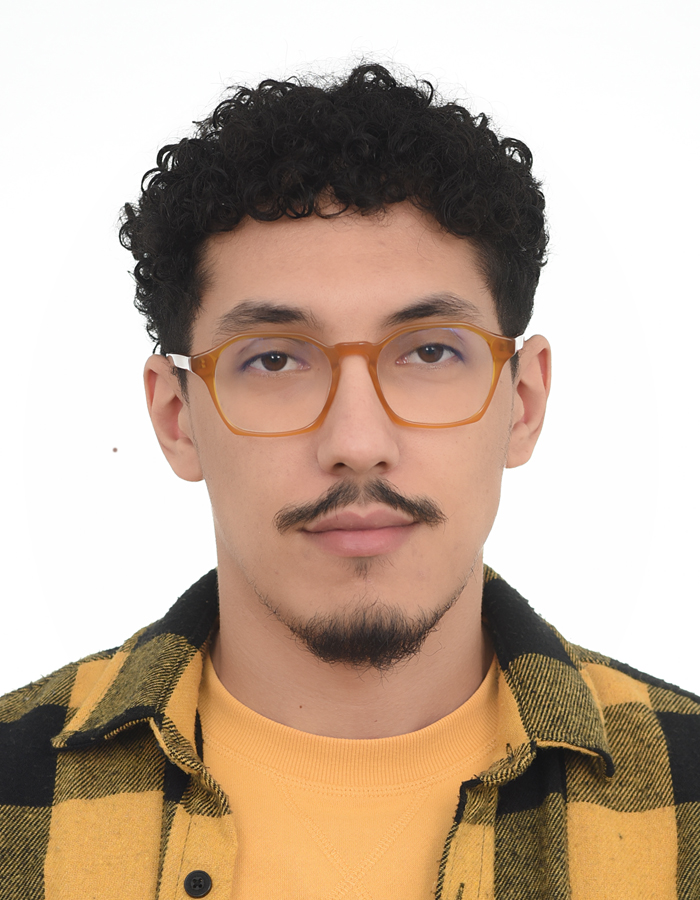
\includegraphics[width=0.85\linewidth]{images/ahmed.jpg}
\end{minipage}%
\hfill
\begin{minipage}[c]{0.84\textwidth}
  \begin{center}
    {\fontsize{20}{22}\selectfont\textbf{Ahmed MAKROUM}}\\
    {\fontsize{13.2}{15.4}\selectfont Ingénieur Data \& Développeur Full-Stack Web/Mobile} \\
    {\fontsize{10.5}{12.3}\selectfont
      \faMobile\enspace +212 664715219 \quad
      \faEnvelope\enspace ahmedmakroum3@gmail.com \quad
      \faHome\enspace Casablanca, Maroc \\
      \faLinkedin\enspace \href{https://www.linkedin.com/in/ahmed-makroum/}{in/ahmedmakroum} \quad
      \faGithub\enspace \href{https://github.com/ahmedmakroum}{github.com/ahmedmakroum}
      \faGlobe\enspace \href{https://ahmedmakroum.github.io/AhmedMakroumPortfolio/}{makroum.me}
    }
  \end{center}
\end{minipage}
\vspace{-10pt}

% PROFIL
\section{\fontsize{11}{12.1}\selectfont Profil}
\vspace{-6pt}
Ingénieur en informatique et réseaux (MIAGE : Méthodes Informatiques Appliquées à la Gestion des Entreprises), avec une solide expertise en génie logiciel, data engineering et développement full-stack. Spécialisé dans la construction de pipelines de données robustes, le développement d’applications web/mobile évolutives et l’intégration de technologies cloud et open source. Apprécié pour sa polyvalence, son esprit d’équipe et sa curiosité continue.

% EXPÉRIENCE
\vspace{-15pt}
\section{\fontsize{11}{12.1}\selectfont Expérience}

\customcventry{03/2025 ‐ Présent}{\href{https://www.allianz.ma}{Allianz Maroc}}{Data Engineer}{}{}{
\begin{itemize}[leftmargin=0.5cm, itemsep=-2pt, topsep=0pt, partopsep=0pt, parsep=0pt]
\fontsize{9.5}{11.2}\selectfont
\item Conception et déploiement de pipelines de données (NiFi, Spark) pour l’extraction, le nettoyage et le chargement depuis les systèmes d’assurance internes.
\item Intégration de sources fragmentées dans un entrepôt PostgreSQL pour un reporting unifié.
\item Création de dashboards temps réel avec Metabase, facilitant l’accès aux données pour les utilisateurs métiers.
\item Développement et maintenance d'une application web de gestion des règlements de santé (Spring Boot, Next.js).
\end{itemize}}

\customcventry{06/2024 ‐ 08/2024}{\href{https://boti.education/}{BOTI School}}{Data Engineer}{}{}{
\begin{itemize}[leftmargin=0.8cm, itemsep=-2pt, topsep=0pt, partopsep=0pt, parsep=0pt]
\fontsize{9.5}{11.2}\selectfont
\item Développement d’un pipeline ETL scalable avec Apache Beam sur Google Cloud.
\item Transformation des logs d’activité en données structurées pour une meilleure analyse comportementale.
\item Production de dashboards automatisés via Looker à destination de la direction.
\end{itemize}}

\customcventry{06/2023 ‐ 08/2023}{\href{https://6solutions.com/}{6solutions}}{Web and Mobile Developer}{}{}{
\begin{itemize}[leftmargin=0.8cm, itemsep=0pt, topsep=0pt]
\fontsize{9.5}{11.2}\selectfont
\item Développement d’une plateforme de consulting multi-services (juridique, médical, financier).
\item Front-end réalisé avec Angular, back-end avec Spring Boot.
\item Conception et déploiement de l’application mobile en Flutter.
\end{itemize}}


\customcventry{07/2022 ‐ 08/2022}{\href{https://estatmar.ma/}{Finso}}{Game Developer}{}{}{%
\begin{itemize}[leftmargin=0.8cm, itemsep=0pt, topsep=0pt]
\fontsize{9.5}{11.2}\selectfont
\item Création d’un jeu éducatif pour enfants sous Unity.
\item Conception de gameplay interactif centré sur l’apprentissage.
\item Optimisation de l’expérience utilisateur et des animations dans un contexte de production réel.
\end{itemize}}}

% PROJETS
\vspace{-13pt}
\section{\fontsize{11}{12.1}\selectfont Projets}
\vspace{-6pt}
\begin{itemize}[leftmargin=0.3cm, itemsep=-2pt, topsep=0pt, partopsep=0pt, parsep=0pt]
    \item \textbf{Portfolio Web Personnel}~--~Site web interactif présentant mes projets, compétences et expériences. (React, Next.js, GitHub Pages)
    \item \textbf{Gestionnaire de Tâches Collaboratif}~--~Application web temps réel pour la gestion d’équipes et de projets. (Spring Boot, React, PostgreSQL)
    \item \textbf{Pipeline ETL Cloud}: Automatisation de l’extraction et du traitement de données volumineuses sur GCP. (Apache Beam, BigQuery)
    \item \textbf{Jeu éducatif Unity}: Développement d’un jeu pour enfants axé sur l’apprentissage interactif. (Unity, C#)
\end{itemize}

% FORMATION
\vspace{-13pt}
\section{\fontsize{11}{12.1}\selectfont Formation}
\vspace{-5pt}
\customcventry{2020 -- 2025}{\href{https://emsi.ma}{\textbf{EMSI – École Marocaine des Sciences de l’Ingénieur}}}{Master MIAGE Ingénierie Logicielle et Réseaux \\ (Méthodes Informatiques Appliquées à la Gestion des Entreprises)}{}{}{}}
\customcventry{Juil. 2024 ‐ Sep. 2024}{\href{https://www.alxafrica.com}{\textbf{ALX Academy}}}{Diplôme associé en Intelligence Artificielle et Prompt Engineering}{}{}{ALX AiCE – Fondamentaux IA}

% CERTIFICATIONS
\vspace{-13pt}
\section{\fontsize{11}{12.1}\selectfont Certifications}
\vspace{-5pt}
\textit{Certifications obtenues via Coursera.}
\begin{itemize}[leftmargin=0.5cm, itemsep=-2pt, topsep=0pt, partopsep=0pt, parsep=0pt]
    \item \textbf{\href{https://www.coursera.org/account/accomplishments/verify/G178XXP17WQA}{Machine Learning with Python}} (IBM)
    \item \textbf{\href{https://www.coursera.org/account/accomplishments/records/M5RKGX36BAVA}{IBM Data Engineering}} (IBM)
    \item \textbf{\href{https://google.com}{Building Scalable Java Microservices with Spring Boot and Spring Cloud}} (Google Cloud)
    \item \textbf{\href{https://www.coursera.org/account/accomplishments/verify/EK5SJM3YM7PX}{Introduction to Big Data with Spark and Hadoop}} (IBM)
    \item \textbf{\href{https://www.coursera.org/account/accomplishments/specialization/B4RCUAYCUG49}{Python for Everybody Specialization}} (University of Michigan)
    \item \textbf{\href{https://www.coursera.org/account/accomplishments/records/G867SJLRFQS2}{Google Business Intelligence}} (Google)
\end{itemize}

% COMPÉTENCES
\vspace{-13pt}
\section{\fontsize{11}{12.1}\selectfont Compétences}
\vspace{-6pt}
\begin{itemize}[leftmargin=0.3cm, itemsep=-2pt, topsep=0pt, partopsep=0pt, parsep=0pt]
    \item Data Engineering : ETL, NiFi, Spark, Beam, PostgreSQL, GCP, AWS
    \item Programmation : C, Python, SQL, Java, TypeScript
    \item Web/Mobile : React, Next.js, Flutter, Spring boot, Apis REST
    \item DevOps : Docker, Kubernetes, Git, CI/CD, Linux
    \item Visualisation : Metabase, Superset, Power BI
    \item Soft Skills : Travail d'équipe, Communication, Adaptabilité
\end{itemize}

% LANGUES
\vspace{-15pt}
\section{\fontsize{11}{12.1}\selectfont Langues}
\vspace{-18pt}
\begin{multicols}{2}
\begin{itemize}[leftmargin=0.3cm, itemsep=-2pt, topsep=0pt, partopsep=0pt, parsep=0pt]
    \item Anglais – Courant
    \item Français – Courant
    \item Arabe – Maternelle
    \item Espagnol – Notions
\end{itemize}
\end{multicols}
\vspace{-6pt}

    % FOOTER
\vspace{0.5em}
\begin{center}
    {\footnotesize\color{gray}
    To learn more about my projects and skills, feel free to check out my~
    \faLinkedin~\href{https://www.linkedin.com/in/ahmed-makroum/}{LinkedIn}~or~\faGithub~\href{https://github.com/ahmedmakroum}{GitHub}.}
\end{center}

\end{document}
